\documentclass[mathserif]{beamer}


\usetheme{Singapore}
%\usepackage{pifont}
\usepackage{color}
\usepackage{rotating}
\usepackage{graphicx}
\usepackage{amsmath}

\newcommand\word[1]{{\textit{#1}}}



\definecolor{rosso}{RGB}{220,57,18}
\definecolor{giallo}{RGB}{255,153,0}
\definecolor{blu}{RGB}{102,140,217}
\definecolor{verde}{RGB}{16,150,24}
\definecolor{viola}{RGB}{153,0,153}
\definecolor{babyblue}{RGB}{0,129,255}
\definecolor{darkgreen}{RGB}{6,148,60}


% BEAMER RELATED DESIGN OPTIMIZATION
\newcommand\highlight[1]{{\usebeamercolor[fg]{structure} #1}}
\setbeamertemplate{navigation symbols}{}
\setbeamertemplate{section in head/foot}{\color{red}{\hfill\insertsectionheadnumber.~\insertsectionhead}}
\setbeamertemplate{section in head/foot shaded}{\color{structure!50}\hfill\insertsectionheadnumber.~\insertsectionhead}
\setbeamertemplate{frametitle}
{
	{\usebeamercolor[fg]{structure} \insertframetitle}\\

	\textit{\footnotesize{\insertframesubtitle}}
}
\newcommand{\changecolor}[1]{
  \setbeamercolor{title}{fg=black}
  \setbeamercolor{frametitle}{fg=black}
  \pgfdeclareverticalshading{beamer@headfade}{\paperwidth}
  {
    color(0cm)=(section in head/foot.bg);%
    color(.95cm)=(#1)
  } 
}




\begin{document}
\changecolor{white}

\begin{frame}[plain]
\begin{center}
\highlight{\large CLS Pre-doc Summer School 2017\\NLU with TensorFlow}\\

\vspace{1cm}
\vfill
\footnotesize
\vspace{0.1cm}
Data Analytics Lab, ETH Z{\"u}rich\\
\vspace{0.1cm}
www.da.inf.ethz.ch\\
\vspace{0.1cm}
florian.schmidt@inf.ethz.ch, yannic.kilcher@inf.ethz.ch\\
\vspace{1cm}
\url{https://github.com/dalab/cls-predoc-nlu-tutorial.git}
\end{center}
\end{frame}


\scriptsize


\begin{frame}{Quick introduction}
	\begin{block}{Now}
		\begin{enumerate}
			\item Tensorflow basics
			\item Constructing a simple model and training it
			\item Monitoring, Printing, Debugging
		\end{enumerate}
	\end{block}
\end{frame}

\section{Tensorflow Basics}


\begin{frame}[fragile]
	\frametitle{Variables and Tensors in Tensorflow}
	\begin{block}{Variables}
		\begin{itemize}
			\item Maintain their state\\
			\item Different methods to create... 
			\begin{verbatim}
			W1 = tf.Variable([[0.1,2.2], [-2.7,0.3]], name = "weights")
			W2 = tf.Variable(tf.zeros([200, 200]), name = "weights")
			W3 = tf.Variable(tf.random_uniform([200, 200], -10, 10), name = "weights")			
			\end{verbatim}
		\end{itemize}
	\end{block}
	\begin{block}{Tensors}
		At every node of the graph, the result of a computation is a tensor.\\

		Tensors have...
		\begin{itemize}
			\item ... a shape, e.g.
			\begin{itemize}
				\item\texttt{\{\}} (scalar)
				\item\texttt{[20]} (20-d vector)
				\item\texttt{[50,10]} (50x10 matrix)
				\item\texttt{[32,3,100,100]} (higher order tensors)
			\end{itemize}
			\item ...a type e.g.\ \texttt{tf.int32}, \texttt{tf.float32}, \texttt{tf.bool}, \texttt{tf.string}
		\end{itemize}
	\end{block}
\end{frame}

\begin{frame}[fragile]
	\frametitle{The graph concept in TF}
		
	
	\begin{itemize}		
		\item Variables
		\item (Input) Placeholders
		\begin{verbatim}
			x = tf.placeholder(tf.float32, [200,10], "input")
		\end{verbatim}
		\item Operations (e.g.\ for matrices \texttt{A,B,C})
		\begin{verbatim}
			C = A - B
			C = tf.matmul(A,B)
			C = tf.nn.relu(A)
		\end{verbatim}
		Common operations include
		
		\begin{itemize}
			
			\item\footnotesize Pointwise: \texttt{tf.mul, tf.add, tf.sigmoid, tf.tanh, tf.nn.relu}
			\item\footnotesize Summing and averaging: \texttt{tf.reduce\_sum, tf.reduce\_mean}		
		\end{itemize}		
	\end{itemize}
\end{frame}


\begin{frame}[fragile]
	\frametitle{Initialization and Sessions}
	  Starting the session fixes the graph and places the ops on devices.
	
	\begin{verbatim}
		x = tf.placeholder(tf.float32, [200,10], "input") # Input placeholder
		W_1 = tf.Variable(tf.zeros([200, 200]), name = "weights")
		hidden_1 = ... # Some deep network here
		hidden_2 = ...
		
		...
		y = tf....     # Network output
		
		# Run graph to get output given an input
		with tf.Session() as session:
		  datapoint = ...  # some np array of size [200, 10]
		  feed_dict = {x : datapoint}	# Map TF placeholders to numpy arrays
		  y_output = session.run(y, feed_dict = feed_dict)   #run the graph
		  
		  print("Output is " + y_output)
	\end{verbatim}
\end{frame}


\begin{frame}[fragile]
	\frametitle{Training}
	Example:
	\begin{verbatim}
		loss = ...   # some scalar tensor
		opt = tf.train.GradientDescentOptimizer(0.01) # here fixed learning rate
		update_step = opt.minimize(loss, global_step)
	\end{verbatim}
	
	See also \url{https://www.tensorflow.org/api_docs/python/train.html}
\end{frame}

\section{Example model}

\begin{frame}{Example: Autoencoder}
	\begin{block}{The Problem}
		\vspace{-0.3cm}
		\begin{align*}
			\text{Given data}&\qquad\mathcal X = \lbrace x_1,\dots,x_n\rbrace\subset\mathbb R^d\\
			\text{and $\tilde d < d$, find}&\qquad f:\mathbb R^d\rightarrow\mathbb R^{\tilde d} \text{\ and\ } g:\mathbb R^{\tilde d}\rightarrow\mathbb R^d\\
			\text{so that for}&\qquad h_i=f(x_i)\in{R}^{\tilde d}\\
			\text{the reconstruction error}&\qquad\sum_i\Vert x_i -g(h_i)\Vert_2^2\  \text{\ is small}
		\end{align*}
	\end{block}
	\vspace{-0.5cm}
	\begin{block}{Neural network approach with single hidden layer}
		\begin{figure}
			\centering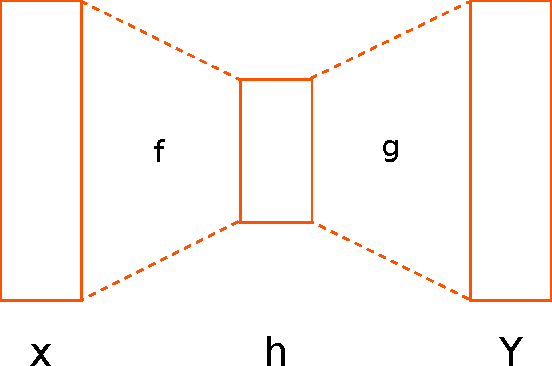
\includegraphics[scale=0.4]{autoencoder.pdf}
		\end{figure}
		\vspace{-0.5cm}
		\begin{align*}
			h &= f(x)=\sigma\left(\mathbf W_\text{enc}x + b_\text{enc}\right)\qquad\text{with $\mathbf W_\text{enc}\in\mathbb R^{\tilde d\times d},\ b_\text{enc}\in\mathbb R^{\tilde d}$}\\
			y &= g(h)=\sigma\left(\mathbf W_\text{dec}h + b_\text{dec}\right)\qquad\text{with $\mathbf W_\text{dec}\in\mathbb R^{d\times\tilde d},\ b_\text{dec}\in\mathbb R^d$}
		\end{align*}
	\end{block}
\end{frame}

\begin{frame}[fragile]
	\frametitle{Example: Autoencoder in TF}
	\begin{verbatim}
d_data = 100        
d_hidden = 30   

# Construct Graph
x = tf.placeholder(tf.float32, [d_data,1], name="input")
  
# Hidden Layer Variables
W_enc = tf.Variable(tf.random_uniform([d_hidden,d_data], -1, 1), name="W_enc")
b_enc = tf.Variable(tf.zeros([d_hidden,1]), name = "bias_enc")
  
W_dec = tf.Variable(tf.random_uniform([d_data,d_hidden], -1, 1), name="W_dec")
b_dec = tf.Variable(tf.zeros([d_data]), name = "bias_dec")
  
# Hidden layer graph
h = (tf.matmul(W_enc, x) + b_enc)

# Output and reconstruction loss
y = (tf.matmul(W_dec, h) + b_dec)
loss = tf.sqrt(tf.reduce_sum(tf.square(x - y)))
  
# Optimizer 
opt = tf.train.GradientDescentOptimizer(0.01)
update_step = opt.minimize(loss)
\end{verbatim}
\end{frame}


\begin{frame}[plain]
	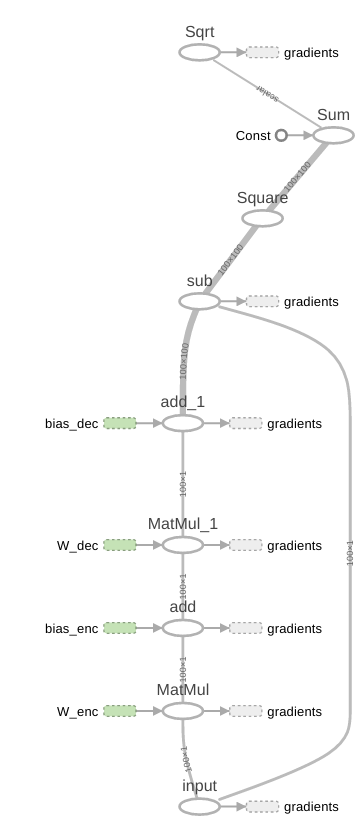
\includegraphics[scale=0.32]{tensorboard-ae-graph.png}
\end{frame}
\section{Monitoring, Printing, Debugging}

\begin{frame}[fragile]
	\frametitle{Printing and Debugging}
	\begin{block}{Printing}
		You cannot access a tensor's content e.g. \texttt{W[0][1]}\\
		Only properties such as \texttt{W.get\_shape()} or \texttt{W.type} are available.
		\begin{itemize}		
			\item Option 1, one-time printing: Run the tensor in a session
			\begin{verbatim}
				W_data = session.run(W)   #get numpy.ndarray
				print(W_data) 
			\end{verbatim}
			\item Option 2, print continuously: \texttt{Print} node
			\begin{verbatim}
				W = tf.Variable(tf.zeros([100,100]),...)
				W = tf.Print(W, [W], message="Entries of W: ")
				X = tf.matmul(W, X)...		# W is still a matrix
			\end{verbatim}
		\end{itemize}
	\end{block}
	


	\begin{block}{Debugging the graph}
		\begin{itemize}
			\item In tensorboard manually check all dependencies in the graph
		\end{itemize}
	\end{block}
	
	See also \url{https://www.tensorflow.org/get\_started/get\_started}
\end{frame}

\begin{frame}[fragile]
	\frametitle{Example: Autoencoder in TF}
	\begin{verbatim}
    data = np.random.rand(d_data, n_datapoints + 1) 
  	
  		 # Train
  	with tf.Session() as session:
    # Initialize variables
    init = tf.initialize_all_variables() 
    session.run(init)
    
    # Do nsteps many SGD update steps
    for i in range(10000):
      datapoint = data[:,np.random.randint(0, n_datapoints)]
      feed_dict = {x : np.transpose([datapoint])}
      session.run(update_step, feed_dict = feed_dict)
      
      # Every now and then test the lost on our hold out datapoint 
      if i % 200 == 0:
        test_point = data[:, n_datapoints]
        feed_dict = {x : np.transpose([test_point])}
        test_loss = session.run(loss, feed_dict = feed_dict)
        print("test loss is %f " % test_loss)

  	\end{verbatim}
\end{frame}


\begin{frame}{Tensorboard}
	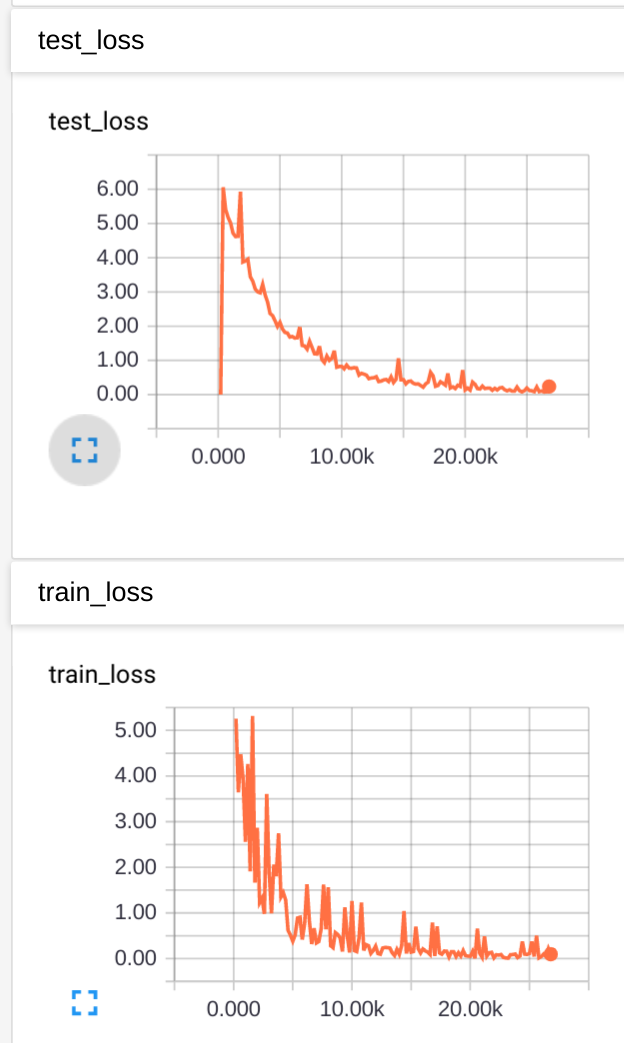
\includegraphics[scale=0.18]{tensorboard.png}
		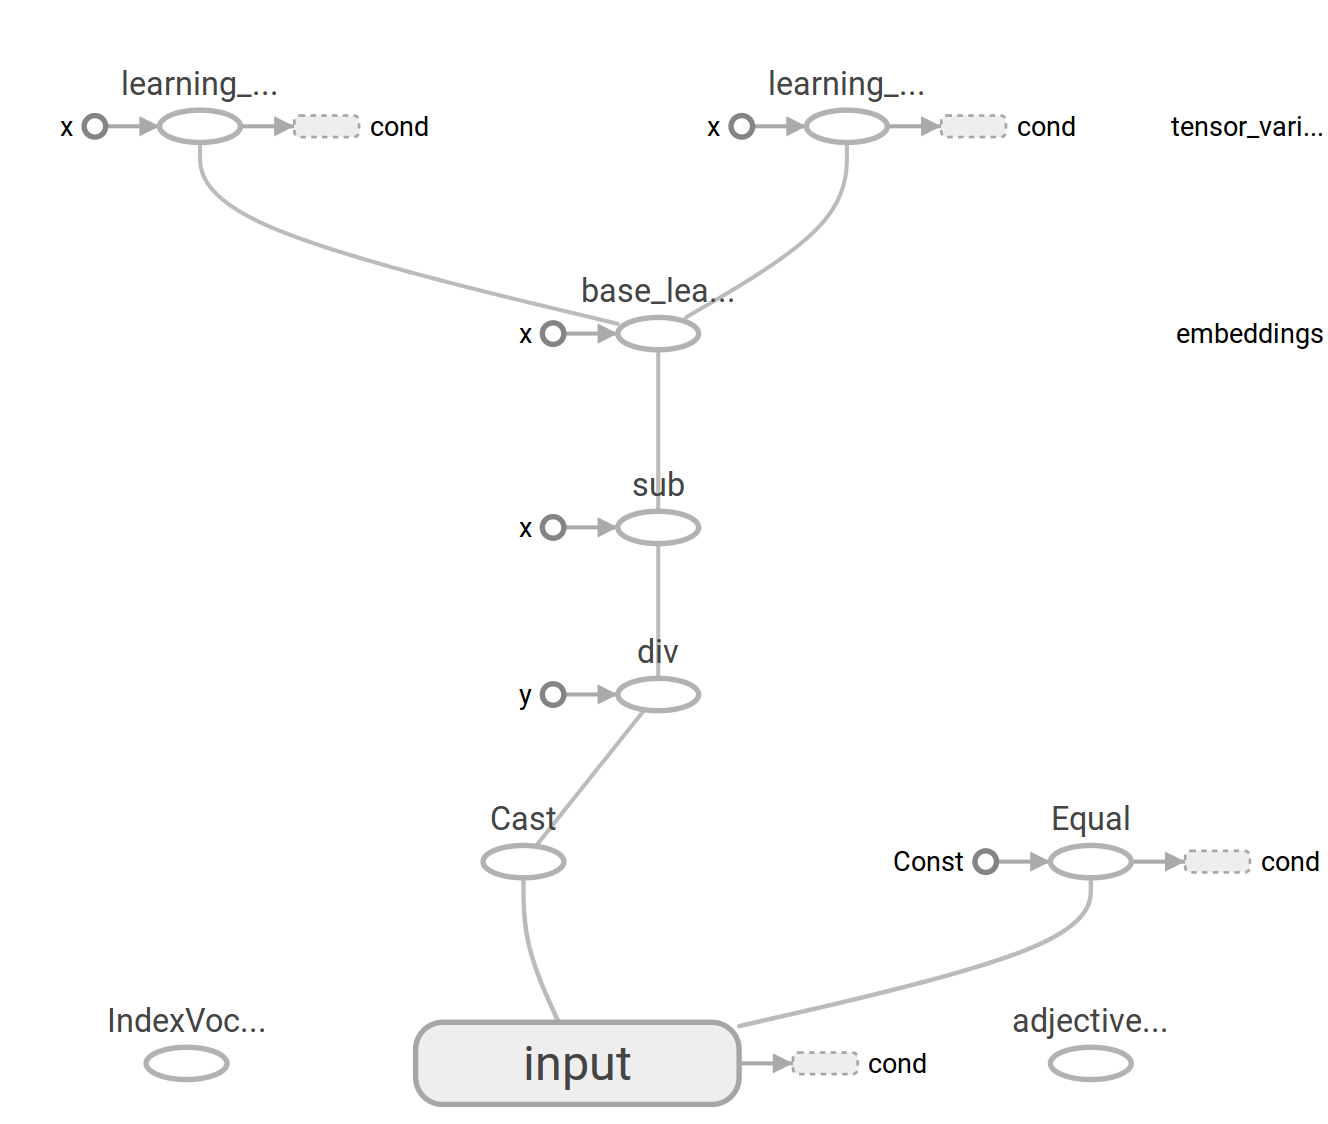
\includegraphics[scale=0.14]{tensorboard-graph.png}

\end{frame}

\begin{frame}[fragile]
	\frametitle{Tensorboard}
	\framesubtitle{How to add a summary}
	For example, track the norm of \texttt{W = tf.Variable(tf.zeros([100,100]),...)}
	\begin{block}{Creating Summaries}
			Once globally:
			\begin{itemize}
				\item Create a summary writer\\ \texttt{summary\_writer =  tf.summary.FileWriter("/my/directory")}
			\end{itemize}
			For this particular summary:
			\begin{itemize}
				\item Get the norm: \texttt{W\_norm = tf.sqrt(tf.sum\_reduce(tf.square(W)))}
				\item Create summary: \texttt{W\_summary = tf.summary.scalar("Norm of W", W\_norm)}
			\end{itemize}
	\end{block}
	\begin{block}{Computing Summaries}
		\begin{itemize}
			\item Merge all summaries: \texttt{summaries = tf.summary.merge([W\_summary,...])}
			\item Fetch the data and turn into a formatted string:\\
			 \texttt{summary\_str = session.run(summaries)}
			\item Send the string to the writer\\
			\texttt{summary\_writer.add\_summary(summary\_str, global\_step)}
		\end{itemize}
	\end{block}
\end{frame}

\begin{frame}{Resources}
	The \textit{How to} and \textit{Tutorials} section on tensorflow.org are actually good resources to recap concepts.\\
	\url{https://www.tensorflow.org/get_started/index.html}\\
	\url{https://www.tensorflow.org/tutorials/index.html}\\
	\vspace{2cm}
	For specific problems, google search often delivers quite useful threads on \url{http://stackoverflow.com} and \url{https://github.com/tensorflow/tensorflow/issues}
\end{frame}

\end{document}




